%% \begin{frame}[t]{Regression Testing to the Rescue}

  \hspace*{-.5in}
  \begin{minipage}{5in}
  \begin{center}

      \begin{minipage}{4.5in}

    \tikzstyle{proc} = [draw, thick, fill=blue!40, text centered, rounded corners]
    \tikzstyle{prochighlight} = [draw, thick, fill=yellow!40, text centered, rounded corners]
    \tikzstyle{procold} = [draw, thick, fill=black!40, text centered, rounded corners]

    \tikzstyle{io} = [ellipse, draw, thick, fill=blue!20]
    \tikzstyle{iohighlight} = [ellipse, draw, thick, fill=yellow!20]
    \tikzstyle{feature} = [draw, thick, fill=orange!40, text centered]  
    \tikzstyle{featureold} = [draw, thick, fill=black!40, text centered]
    \tikzstyle{special} = [draw, thick, fill=purple!40, text centered, rounded corners]    

    \begin{figure}

    \begin{center}

      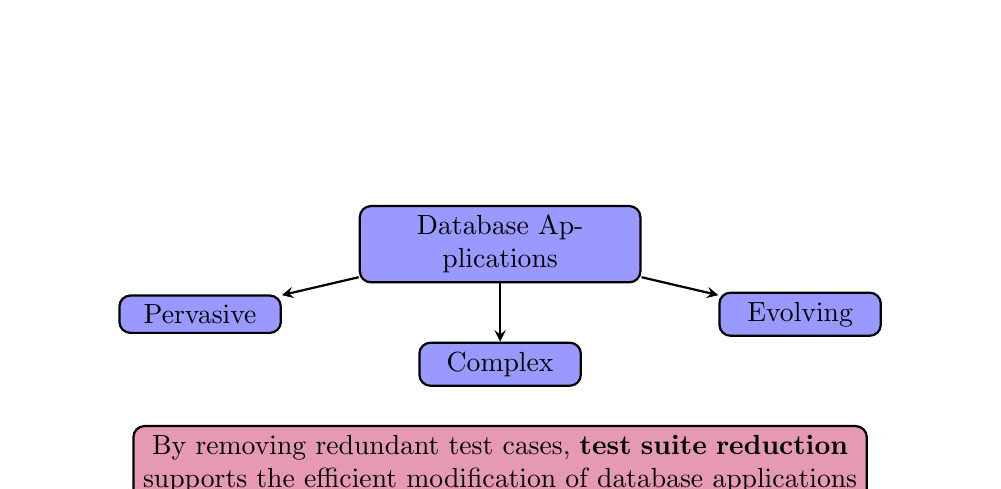
\begin{tikzpicture}[node distance=0cm, auto,>=stealth, thick]
	
        \path[use as bounding box] (-2,3.5) rectangle (10,-2);

        % Computer Software
    	\path[->]<1-> node[proc, text width=22ex] 
        (Software) at (4,.75) {Database Applications};

        % Pervasive
        \path[->]<1-> node[proc, right of=Software,  
                      yshift=-.35in, xshift=-1.5in, text width=12ex] 
                      (Pervasive) {Pervasive}
        (Software) edge node {} (Pervasive);

        % Complex
        \path[->]<1-> node[proc, below of=Software,  
                      yshift=-.6in, xshift=0in, text width=12ex] 
                      (Complex) {Complex}
        (Software) edge node {} (Complex);

        % Evolving
        \path[->]<1-> node[proc, right of=Software,  
                      yshift=-.35in, xshift=1.5in, text width=12ex] 
                      (Evolving) {Evolving}
        (Software) edge node {} (Evolving);

        % An assertion
        \path[->]<1-> node[special, below of=Software,  
                      yshift=-1.1in,text width=60ex] 
                      (Assertion) 
        {By removing redundant test cases, {\bf test suite reduction}
          supports the efficient modification of database applications};

 	\end{tikzpicture}
	
        \end{center}

        \end{figure}
      
      \end{minipage} 

  \end{center}
  \end{minipage}

%% \end{frame}

